\chapter{The \Tigris language}
\Tigris 是一个注重可读性与语法统一性的灵活的，纯函数式静态类型的语言。它从 Lean、OCaml 和 Haskell 汲取灵感。

\section{词法惯例}
在下文我们用一套修改版的 BNF（Backus-Naur Normal Form，误和 ABNF 混淆）来表示表层语法。修改过的 BNF 可以在其
右手侧（RHS）接受 POSIX 正则表达式中的 \texttt{+*[\,\^\;]}.
{\setlength{\parskip}{-1em}
  \paragraph*{文本编码} Tigris 源代码应当是 UTF-8 编码的文本文件。
  \paragraph*{空白字符} 包含空格（spaces）、制表符（tabs）、CR/LF。空白字符会被忽略，因而
  不影响程序的语义。\footnote{在定理证明器一侧并非如此。}
  通过使用空白字符，相邻的标识符、字面量以及关键字可以被隔开，而不被算入同一个标识符中。
  \paragraph*{注释} 指以 \texttt{--}（Lean/Haskell/Lua 风格）或以 \texttt{NB.}（J 风格）开头的\emph{单行}注释。
  与空白字符相同，注释也会被词法分析器忽略。注意目前并不支持多行注释。
}
\paragraph*{标识符} 几乎和 Ocaml/Haskell/Lean 一致。
\begin{definition}[标识符]\label{def:ident} 由以下 BNF 文法给出
  \begin{minted}{bnf}
  <ident>        ::= (<letter> | _) <rest>*
  <upper-ident>  ::= <uppercase> <rest>*
  <lower-ident>  ::= <lowercase> <rest>*
  <letter>       ::= <upper-letter> | <lower-letter>
  <rest>         ::= <letter> | 0..9 | _ | ' | ! | ?
  <lower-letter> ::= a..z
  <upper-letter> ::= A..Z
  \end{minted}
\end{definition}

为了化简语法分析，标识符是否由大写字母开头具有语义（后述），而以 \texttt{'!?} 结尾的标识符
则不做区分。后者是为了允许一些常见的代码风格，例如以 \texttt{?} 结尾表示一个可空的值/函数（\mintinline{Haskell}|Option a|）、
以 \texttt{!} 结尾表示一个函数可能抛出错误或造成非本地返回（non-local exiting）。

{\setlength{\parskip}{-1em}
  \paragraph*{整数字面量} \mintinline{bnf}{<intlit> ::= ("-" | "+")? 0..9+}，十进制且支持大数。
  \paragraph*{字符串字面量} \mintinline{bnf}{<strlit> ::= "[^"]+"}
  \paragraph*{保留符号及关键字} 由表 \ref{tab:reserved-symbols} 给出；
  词法分析的歧义按照\emph{最长匹配}原则进行处理。
}

\begin{table}
  \centering
  \caption{保留符号及关键字}\label{tab:reserved-symbols}
  {\tt
    \begin{tabular}{@{}lllllllllll@{}}
      \toprule
      \multicolumn{4}{c}{\textrm{符号}}                & \multicolumn{7}{c}{\textrm{关键字}}                                \\ \midrule
      | & -\textgreater{} & ;; & =\textgreater{} & mutual & infixl & infixr   & match & then   & let     & fun \\
      , & \_              & :  & ∀          & extern & class  & forall   & data  & prefix & postfix & in  \\
      &                 &    &                 & type   & with   & instance & else  & and    & rec     & if \\ \bottomrule
  \end{tabular}}
\end{table}

\section{值}
\emph{值}（value）是不能够再消去（化简）的表达式，可以理解为一个\emph{范式}。
用大步操作语义（big-step operational semantics）表示为
\(\inmark{v, \sigma} \Downarrow \inmark{v}\) 其中 \(v\) 是以下其中之一：
{\setlength{\parskip}{-1em}
  \paragraph*{整数字} 整数的范围取决于后端。在我们的实现中，无论是 SBCL 后端，还是 Lean 编写的
  解释器，都支持可变精度数字，亦即大数运算，因而不存在相对底层语言的\texttt{u32}、\texttt{i64}等等数据类型。
  \paragraph*{字符串} 是字符的无穷序列。其长度限制取决于后端。在我们的实现中，SBCL 后端支持长达 $2^{45}$ 的字符串。
  \paragraph*{元组} \(n\)-元组（tuple）通常写作 \((v_1,\dots,v_n)\).\footnote{元组在实现中是特殊对待，并非由常规的 $\mathsf{Prod}$ 编码。}
  \paragraph*{结构体} 亦称\emph{记录}（record）。是归纳类型/代数数据类型（inductive/algebraic datatype, ADT）的语法糖，字面量写作
  \(\{\textit{field}_1 = v_1,\dots,\textit{field}_n=v_n\}\).\footnote{而类型类的实例又是结构体的语法糖。}
  考虑到潜在的大重构问题，当前版本的 Tigris 只实现了\emph{伪类型制导}句法分析。因而对具有相同栏位（field）的
  结构体来说，无论其类型如何，都会抛出一个句法分析歧义警告（ambiguous parsing warning），但该警告可被
  类型标注（包括后述的模式亦是如此）消除：\footnote{
    因为它是由句法分析器处理而并非类型检查器，该类型标注必须置于结构体字面量上。
}}
\begin{minted}[frame=single]{Haskell}
type Point  = {x : Int, y : Int} -- Point' 定义和 Point 相同
-- ambiguous record literal (using default 'Point'),
-- candidates are [(Point, #[x, y]), (Point', #[x, y])]
let _ = {x = 1, y = 2}
let _ = ({x = 1, y = 2} : Point') -- 成功
\end{minted}
对于栏位有重叠的部分，我们用最长匹配规则来区分（其中 \texttt{x} 被推断为 \texttt{Point}，\texttt{y} 被推断为 \texttt{Point3D}）：
\begin{minted}[frame=single]{Haskell}
type Point3D = {x : Int, y : Int, z : Int}
let (x, y) = ({x = 1, y = 2}, {x = 1, y = 2, z = 3})
\end{minted}
{\setlength{\parskip}{-1em}
  \paragraph*{构造值} 指的是通过某一归纳类型的\emph{值构造子}（value constructor，简称\emph{构造子}，constructor）
  构造出的值，英文亦作\emph{variant}. 构造子类似函数，但他们也可以不接收任何参数：对某构造子 $C_i$，其构造值
  一定是 $C_i$ 或 $C_i\ \textit{fid}_1\ \cdots\ \textit{fid}_n$. 内置的构造值包括
  $
  \{\mathsf{true}, \mathsf{false}\} : \mathsf{Bool};\;\;\{\mathsf{()}\} : \mathsf{Unit}
  $.
  \paragraph*{函数} 指从值到值的映射，细节后述。
}
\section{标识符}
定义 \ref{def:ident} 规定的标识符用于指代某一\emph{语言对象}。表 \ref{tab:ident-case} 展示了
不同类别的语言对象的大小写规定。

\section{类型表达式}
\begin{definition}[类型表达式] 由以下 BNF 给出
\begin{minted}{bnf}
<type-expr>   ::= <type-app> (-> <type-expr>)?                 arrow type
<type-atom>   ::= <ident> | "(" <type-expr> ")"                parenthesized
                | <type-ctor> | <type-args>
                | sepBy("*" | "×", <type-expr>)                product type
<type-app>    ::= <type-app>? <type-atom>                      type application
<type-ctor>   ::= <upper-ident>
<bound-ty>    ::= <lower-ident>
<type-binder> ::= <bound-ty> | "(" <bound-ty> : <intlit> ")"   type binder
<type-args>   ::= <bound-ty> | <type-expr>                     type argument
<qualified>   ::= "[" sepBy1(",", (<bound-ty> | <type-ctor>) <type-expr>+) "]"
<scheme>      ::= (FORALL <type-binder>+)? <qualified>? "," <type-expr>
FORALL        ::= forall | ∀
\end{minted}
\end{definition}
需要注意，对于并列式\footnote{
  并列式指语法上不需要括号的函数\emph{应用}/调用。例如 \texttt{f 1 2} 表示将 \texttt{1, 2}两参数传给 \texttt{f} 并调用之。
  这一语法差异看似简单，实际上有重大差异：函数式语言具有的柯里化（后述）特性使得 \texttt{f 1 2} 比 \texttt{f(1, 2)} 更
  符合语义，因为后者等于向 \texttt{f} 传一个元组 \texttt{(1, 2)}. 这是 ML 系函数式语言的共性，但在 Ruby、Perl/Roku 等语言中
  也有出现，读者可以把其类比为 Shell 命令的调用。而从句法分析的角度考虑，并列式语法的实现
  与中缀运算符一致，但其“算符”是空白字符，因而有下方的优先级表。
}的类型应用（juxtapositional type application）\footnote{
  在实现上，类似 Haskell 2010 Report 中的 a/b-type.
}、
积类型和箭头类型，表 \ref{tab:tyoperator-prec} 给出了其优先级（越高者越先）与结合性。
\begin{figure}
  \centering
  \begin{subfigure}[t]{0.5\textwidth}\centering
    \caption{不同类别标识符的大小写差异}\label{tab:ident-case}
    \begin{tabular}{@{}lr@{}}
      \toprule
      \textbf{类别}             & \textbf{首字母} \\ \midrule
      值               & 任意          \\
      构造子         & 大写    \\
      类型构造子    & 大写    \\
      结构体栏位        & 任意          \\
      约束的类型变量 & 小写    \\ \bottomrule
    \end{tabular}
  \end{subfigure}%
  \begin{subfigure}[t]{0.5\textwidth}\centering
    \caption{类型运算符结合性}\label{tab:tyoperator-prec}
    \begin{tabular}{@{}lr@{}}
      \toprule
      \textbf{运算符}                     & \textbf{结合性} \\ \midrule
      类型应用             & 左         \\
      积类型 (\(\ast\))             & 右         \\
      箭头类型 (\(\to\)) & 右 \\ \bottomrule
    \end{tabular}
  \end{subfigure}
  \caption{大小写规范及运算符结合性}
\end{figure}

\paragraph*{类型变量}\label{fn:HKT} 亦称 TV（type variables），是小写字母开头的标识符。类型变量的\emph{类型}，
即\emph{类型的类型}（kind）是由用户显式提供的，因为目前我们并未实现 TV 的类型推断（kind inference）。
一个记作 \((\alpha : n)\) 的 TV 有类型 \(\mathbf{Type}\to \mathbf{Type}\)，否则默认为 $\mathbf{Type}$.
但因目前我们不允许柯里化的高阶类型存在，\((\alpha : 2)\) 实际上是 \(\mathbf{Type}\times\mathbf{Type}\to\mathbf{Type}\).
因而在称谓上，我们应当使用\emph{元数}（arity）一词而非 kind. 在数据类型定义中，TV 必须是被约束（bound）的，其约束位置可以是
类型构造子的参数位置，或是右手侧的全称量词 $\forall$（forall）中。
读者应当注意到，类型表达式的合法性检查（validity checking）基本在句法分析阶段完成，也就是说，若存在某一 TV 是自由变量（free variable），
编译器会抛出句法分析错误。

在用户接触到的 TV 之外，实现中，编译器存在以下两种具有特殊含义的 TV：

元变量（metavariables），亦称 MV，记作 \texttt{?m.N} 其中 \texttt{N} 是计数器的数字。元变量指代某一未知类型，且必须被
某一类型所实例化（instantiation）\footnote{
  “实例化”一词在本文中经常使用，但该词的具体含义并没有清晰的定义：有时，我们用这词指代特殊化（specialization），
  指 TV 被\emph{实际}（concrete）类型所实例化；有时，我们只用其指代 TV 的替换（substitution）操作。
}
、或在离开作用域时被 HM 类型系统的自动泛化机制所泛化。无论如何，MV 不应当在最终的模式（scheme）\footnote{
  与上面的“实例化”一词相同，“模式”一词，既指代模式匹配中的模式（pattern），亦指代公理模式（此处为类型模式）中的模式（scheme）。
  虽然这容易造成歧义，但两个概念相隔甚远，读者应当能自行区分其具体意思。
}
中出现。

Skolem TV\footnote{纪念挪威数学家 Thoralf Skolem，主要研究数理逻辑与集合论。}，亦称 skolems，记作 \texttt{?sk.a} 其中 \texttt{a} 指代
原始 TV。Skolems 由 skolemization 过程产生，这些 TV 实际上由类型构造子编码\footnote{在实现中，我们用 \texttt{TCon} 编码，避免错误的合一化。}，并且
\emph{绝对不}应被实例化。这使得类型检查器能够查出更多的类型错误，考虑

\begin{minted}[escapeinside=\%\%,frame=single]{lean4}
instance : Functor Option =
  { map -- %$\forall\alpha,\beta.\ (\alpha\to\beta)\to\mathsf{Option}\ \alpha\to\mathsf{Option}\ \beta$%
    | f, None => None
    | f, Some a => Some a} -- [ERROR] Can't unify type ?sk.a with ?sk.b.
\end{minted}

上述例子非法：根据 \texttt{map} 的模式的含义，类型变量 \texttt{a} 和 \texttt{b} 应当相互独立，即 $a \not\sim b$，
其中 $(\sim)$ 算符表示合一化：
在 \texttt{map} 函数体内，两者被 skolemize，不能相互用自身实例化对方。这里，从 \texttt{map} 正确的语义来看，
我们猜想用户应是忘记应用 \texttt{f}，即第二个分支应是 \texttt{Some (f a)}。
即便允许这样的代码，其语义也不正确：但现在可通过 skolems 在编译期捕捉到这一错误并回报给用户。
Skolems 所具有的特殊性质称为\emph{刚性}（rigid），在后文我们会见到不仅仅是 Skolems 具有刚性，但其是最具代表性的。

{\setlength{\parskip}{-1em}
  \paragraph*{函数类型}
  表达式 \(ty_1\to\cdots\to ty_n\) 表示一个从 \(ty_1,\dots,ty_{n-1}\) 到 \(ty_n\) 的函数的类型。
  \paragraph*{积类型}
  表达式 \(ty_1\times\cdots\times ty_n\) 表示一个具有类型为 \(ty_1\times\cdots\times ty_n\) 的元素的元组的类型。
  \paragraph*{构造类型} 与构造值相似，可看做类型层面的值。\footnote{在这里我们仍然清晰地区分类型与值，但这一界限在后文的基于依赖类型的定理证明器中愈发模糊。}
  正如同 TV，类型构造子同样具有元数，而元数为 0 的类型构造子其自身即是类型，构成一个类型表达式。
  但与构造子不同，类型构造子必须完全应用（fully applied），这一特性与工业语言中的函数相似。
  \paragraph*{不定递归类型}\label{para:equirecursive} 会被类型检查器拒绝，因此
  类型检查器无法推断诸如程序 \mintinline{ocaml}|fun x -> x x| 的类型，且一个特殊的错误信息会被抛出。
  这是为了提高类型系统的合理性，因为不定递归类型的方程式无解，或者说其解是一个无限增长的树形结构。
  允许这种类型的存在，就可以构造不动点组合子（fixpoint combinator），其中又以 \texttt{Y} 组合子最为著名（以下是其中一种实现）：
  \begin{equation}
    \mathsf{Y}\ f = f\ (\mathsf{Y}\ f) : \forall \alpha.\;(\alpha\to\alpha)\to\alpha,
  \end{equation}
  将其应用到恒等函数（identity）函数上 $\mathsf{Y}\ \mathrm{id}_\alpha$ 得到类型 $\forall \alpha. \alpha$.
  出现这一类型的\emph{值}是非常危险的，因为该类型可以被实例化到任意一个类型上，即该值具有任意类型，可以是
  整数，也可以是字符串等等。更危险的问题来源于后文 Tigrisd 定理证明器的理论基础 Church-Howard 同构（isomorphism），
  在逻辑上，存在这样的类型（这样的命题成立）可以导出任意命题成立，这显然是大错特错的。而即便我们只禁止这种情况，
  诸如 $\alpha\sim\tau$ 其中 $\alpha\in\tau$ 的合一化也是不合理的，因而我们不允许这种类型的存在。
}
\section{模式}
模式匹配的模式是一个\emph{指令模板}，用于解构（destructure）某种\emph{形状}的数据结构。如果
用户自定义运算符（后述）被绑定到构造子上，则该运算符亦自动作为新的模式（语法糖）出现，提高代码可读性。
无论何种模式，在句法分析期其都将被解糖至以下若干\emph{基本}模式中：
\begin{definition}[模式] 由以下 BNF 给出
\begin{minted}{bnf}
<pat>       ::= <pat-left> <infix-op> <pat>         infix operator enriched
              | <pat-left>
              | <prefix-op> <pat>                   prefix operator enriched
              | <pat> <postfix-op>                  postfix operator enriched
<pat-left>  ::= <pat-atom>
              | <ctor> many1(<pat-atom>)            variant
<pat-atom>  ::= <lower-ident>                       variable
              | <ctor>                              constructor
              | "_"                                 wildcard
              | "{" sepBy1(",", <pat-field>) "}"    record pattern
              | "(" sepBy1(",", <pat>) ")"          product pattern
              | "(" <pat> : <type-expr> ")"         ascribed pattern
              | <literal>
<pat-field> ::= <field> = <pat>
\end{minted}
\end{definition}
注意某一构造子模式的元数必须与其子模式（sub-pattern）的数目相等，即在这个上下文的构造子
必须是完全应用。
表 \ref{tab:patoperator-prec} 展示了 Mixfix（即前缀、中缀、后缀）运算符具有的优先级（越高者越先）。
\begin{table}
  \centering
  \begin{tabular}{@{}ll@{}}
    \toprule
    \textbf{运算符}                & \textbf{结合性} \\ \midrule
    构造子应用（constructor application） & 左          \\
    前缀算符（prefix operator）         &               \\
    后缀算符（postfix operator）       &               \\
    中缀算符（prefix operator）         & 左          \\
    中缀算符          & 右         \\ \bottomrule
  \end{tabular}
  \caption{算符在模式中的优先级}\label{tab:patoperator-prec}
\end{table}

下面叙述各基本模式。

\paragraph*{变量与通配符模式} 将一个标识符与值关联起来，例如 \mintinline{ocaml}|let fst (x, _) = x|.
与其他语言不同，模式不一定是线性的，即单个变量在一个模式中可以绑定多次，且新绑定覆盖旧绑定。但是，应当注意可能的
语义问题：
\begin{minted}[frame=single]{lean4}
let prodEq : ∀a b, a × b → Bool
  | (x, x) => true
  | (x, _) => false -- Found redundant alternatives at 2)  #[(x, _)]
\end{minted}
第一个分支并非测试元组两个元素是否相等，这是显然的：给定任意模式，没有固定的方法测试某一数据结构的两部分是否相等。
要测试相等，应当利用与类型类 \texttt{Eq} 相关联的 \texttt{(=)} 方法（method）。

\paragraph*{字面量模式} 可用于测试字面量是否相等：
\begin{minted}[frame=single]{lean4}
let strToBool : String → Bool = fun
  | "true"  => true
  | "false" => false
\end{minted}
\paragraph*{括号括住的模式} 在混有运算符的模式中起作用：
\begin{minted}[frame=single]{haskell}
type List a = Nil | Cons a (List a) ;; infixr 90 "::" => Cons
let f1 (x :: y :: _)   = (x, y)
let f2 ((x :: y) :: _) = (x, y)
\end{minted}
注意 \texttt{f1} 与 \texttt{f2} 相差甚远（因为用户自定义的 \texttt{(::)} 算符是右结合），
这在编译器自动生成的 \Tigris System F IR 很显然:
\begin{minted}[ignorelexererrors=true]{ocaml}
let (::) : ∀ α, α → List α → List α = (Λ α. Cons@α)
let f1 : ∀ α, List α → α × α =
  (Λ α. fun ?x₀ : List α => match ?x₀ with | Cons x (Cons y _) => (x , y))
let f2 : ∀ α, List (List α) → α × List α =
  (Λ α. fun ?x₀ : List (List α) => match ?x₀ with | Cons (Cons x y) _ => (x , y))
\end{minted}
就如同数学中使用括号提高某个项的运算优先级，自然，在模式中使用括号亦如此。
\paragraph*{构造模式} 有格式 \(C_i\ p_1,\dots,p_n\)：
它匹配所有自 \(C_i\) 构造出，且其参数又满足子模式 \(p_1,\dots,p_n\) 的构造值。当参数与子模式数量不匹配时，
编译器会抛出元数不匹配错误。
\paragraph*{元组模式} 有格式 $(p_1,\dots, p_m)$，因为元组可以看成是由\emph{二元逗号构造子}$(-,-)$构成的构造模式，
而该二元构造子又可看作是右结合的中缀运算符，因而元组、元组模式都是右结合的。
\paragraph*{结构体模式} 与结构体字面量相似，遇到具有相同栏位的模式时会产生句法分析歧义并报警。
结构体是归纳类型的语法糖，结构体模式则是构造模式的语法糖。因而，可以用常规的构造模式去解构之：
\begin{minted}[ignorelexererrors=true,frame=single]{lean4}
class Functor (m : 1) = {map : forall a b, (a → b) → m a → m b}
let getMap (Functor f) = f
\end{minted}

\section{表达式}
表达式是 \Tigris 的核心。非正式地，为了方便后文的描述，我们定义以下元变量：
\begin{table}[H]
  \begin{tabularx}{\linewidth}{@{}lX@{}}
    \toprule
    \textbf{符号}     & \textbf{定义}   \\ \midrule
    \(p_i\) & 表示模式匹配中的第 \(i\) 个模式；          \\
    \(C_i\)         & 表示归纳类型的第 $i$ 个构造子；          \\
    \(e, e', e_i\)             & 表示任意表达式，其值视给定的上下文（环境）而定；   \\
    \(v, v', v_i\)               & 表示值；          \\
    \(a, b, c, d, x, y, z, w\) & 表示标识符；         \\
    \(f, g, h\)          & 表示标识符，在语义上，表示函数；           \\
    \(\sem{}\)            & 是黑板风格字体，在元语言中普通分界符用光时用作分界符； \\
    希腊字母   & 基本表示类型。若其上有一横杠 \(\bar{\alpha}\) 则表示一个序列，并有隐式编号 \(1,\dots,i\). \\ \bottomrule
  \end{tabularx}
\end{table}
任一 \Tigris 表达式，总是将经过足够多的变换操作而被翻译到其核心代数 \texttt{Expr} 中。
以下给出表达式的 BNF 语法规格。
\begin{definition}[表达式] 由以下 BNF 给出
\begin{minted}{bnf}
<expr>        ::= <expr-infix>
                | (<expr-infix> : <type-expr>)                  ascription
<expr-infix>  ::= <expr-left> <infix-op> <expr-infix>           infix operator
                | <prefix-op> <expr-left>                       prefix operator
                | <postfix-op> <expr-left>                      postfix operator
                | <expr-left>
<expr-left>   ::= fun ( <expr-binder>+ ARROW <expr>             lambda abstraction
                      | <expr-match>)
                | let "rec"? <pat'> = expr in <expr>            pattern matching let
                | let "rec"? <let-binder>
                  sepBy("and", <let-binder>)                    let(rec) expression
                  in <expr>
                | if <expr> then <expr> else <expr>             conditional
                | rec <expr>                                    fixpoint; deprecated
                | match sepBy1(",", <expr>) with <expr-match>   pattern matching
                | <expr-funapp>
<expr-funapp> ::= <expr-funapp>? <expr-atom>                    function application
<expr-atom>   ::= <literal>
                | <expr-ctor>
                | <lower-ident>                                 variables
                | "(" sepByN(",", <expr>) ")"   where    N = 0  unit
                                                         N = 1  parenthesized <expr>
                                                         N ≥ 2  product
                | "{" sepBy1(",", <expr-field>) "}"             record literal
<expr-ctor>   ::= <upper-ident>                                 constant constructors
<expr-match>  ::= ("|" sepBy1(",", <pat>) ARROW <expr>)+        pattern match body
<expr-field>  ::= <field> = <expr>
<expr-binder> ::= <id> | <pat'>                                 binders
<pat'>        ::= "(" <pat> ")"                                 parenthesized <pat>
                | <literal>                                     except literal patterns
<let-binder>  ::= <pat'> = <expr>                               single-pattern binding
                | <ident> <expr-binder>* <type-expr>? <let-rhs> value/function binding
<let-rhs>     ::= "=" <expr> | <expr-match>                     let binding RHS
<literal>     ::= <intlit> | <strlit> | "true" | "false"
ARROW         ::= "=>" | "->"
\end{minted}
\end{definition}
\paragraph*{基本表达式} 指的是在 \texttt{<expr-atom>} 中列出的所有语法，加上函数简写的语法糖。
\subparagraph*{函数简写语法} 指的是受 Lean 启发的括号语法糖。在括号内，所有的下划线（\texttt{\_}）或
中点（$\cdot$）会按语法树的前序遍历（preorder，即 DFS）被翻译到函数的绑定位置（function binder）。这类似 Haskell 的
运算符分割（operator sectioning）语法糖。我们的语法糖仍遵守运算符的先后顺序，如图 \ref{code:func-shorthand}.
\begin{figure}[H]
  \centering
  \begin{subfigure}{0.5\textwidth}\centering
\begin{minted}{lean4}
  (_ + 1)
  (_ + 1 * 2 / _)
  (id _)
\end{minted}
    \caption{函数简写}
  \end{subfigure}%
  \begin{subfigure}{0.5\textwidth}\centering
\begin{minted}{lean4}
  fun x   => x + 1
  fun x y => x + 1 * 2 / y
  fun x   => (id : forall a, a -> a) x
\end{minted}
    \caption{解糖结果}
  \end{subfigure}
  \caption{函数简写语法糖的对比}\label{code:func-shorthand}
\end{figure}
被括号括起的表达式亦可以添加类型标注，如上面的例子所示。

\paragraph{柯里化的函数应用与定义}
函数形式的值（functional value）是柯里化的\footnote{构造子与函数构成所有函数形式的值集合的划分。}：多元函数无非是嵌套
着的一元函数（因而除去最内层之外，其余嵌套函数都是高阶函数，即返回值是函数的函数）。也就是说，
函数的部分应用（partial application）是合法且在函数式编程实践中经常被使用的。请读者回想前面我们提到的并列式函数应用语法，体会这一语法之于
柯里化的必要性：常规语法 \texttt{f(1,2)} 隐含地告诉用户该函数必须完全应用，而 \texttt{f 1 2} 则淡化了这一信息（其在 JS 等语言中的等价写法是 \texttt{f(1)(2)}，较为繁琐），用户使用部分应用 \texttt{f 1}
亦不在语感上违和。
而实际上，\Tigris 的函数定义可以看作是普通工业语言的超集，函数 \texttt{f (x, y)} 表示一接收2-元组的一元函数，在语义上等价于需要
完全应用，可用于模拟工业语言的函数定义与应用，虽然这种模式并不常用。
{\setlength{\parskip}{-1em}
  \subparagraph{函数应用} 靠左结合，使用多个表达式并列的语法。此外，\Tigris 是按值调用（call-by-value，CBV），
  若求 \(e\ e'\)，首先求 \(e\) 并确保其是一函数形式的值，其次求 \(e'\).
  \subparagraph{函数定义（Lambda 抽象）} 具有以下两种形式:
  \begin{align*}
    &\mathbf{fun}\;
    \vert\ p_{1,1},\dots,p_{1,m}\Rightarrow e_1\vert\cdots\vert\ p_{n,1},\dots,p_{n,m}\Rightarrow e_{n} \numberthis \label{eqn:fun-1}\\[-6pt]
    &\mathbf{fun}\ p_1\cdots p_m\Rightarrow e \numberthis
  \end{align*}
  而上述两种形式无非是以下形式的语法糖，且与之恒等：
  \begin{equation}
    \begin{aligned}
      \mathbf{fun}&\ x_1\Rightarrow\cdots\mathbf{fun}\ x_n\Rightarrow\\[-10pt]
      &\mathbf{match}\ x_1,\dots,x_m\ \mathbf{with}\\[-10pt]
      &\vert\ p_{1,1},\dots,p_{1,m}\Rightarrow e_1 \\[-5pt]
      &\vert\ \overbrace{p_{2,1},\dots,p_{2,m}\Rightarrow e_{2}}^\textrm{这之下仅适用形式 (\ref{eqn:fun-1})}\\[-10pt]
      &\vdots\\[-10pt]
      &\vert\ p_{n,1},\dots,p_{n,m}\Rightarrow e_{n}
    \end{aligned}
  \end{equation}
  语法上的直觉感受告诉我们，最简形式（canonical）的 Lambda 抽象只接受一个参数，多参数函数本质上是多个单参数函数的嵌套，
  这就是柯里化的要义。
}
\paragraph{Let-绑定\&表达式} 与大多数语言区分值定义与函数定义、全局定义与局部定义的做法不同，作为函数式语言的 \Tigris 将函数
视作头等公民，与其他值待遇相同：无论是传统意义上的值或函数、全局与否的定义，全部通过 Let 或 Letrec 进行绑定——
语法构造 Let/Letrec 将标识符与值关联起来，作用域为本地或全局。

{\setlength{\parskip}{-1em}
  \subparagraph*{命名规则（Nomenclature）} 我们规定，“Let-绑定”（let-biding）描述上述 BNF 语法中的 $p_n = e_n$ 部分，
  \texttt{and}-分支则是隐含存在的（除非显式说明不存在）；“Let-表达式”（let-expression）则在这之上
  包含程序主体部分 \texttt{in <expr-body>}.
  \subparagraph*{本地非递归定义} 语法构造 $\mathbf{let}\ p_1 = e_1\ \mathbf{and}\cdots\mathbf{and}\ p_n = e_n\ \mathbf{in}\ e$ 首先
  并行\footnote{理论上的（在类型检查器中）；实际行为取决于后端。Cf. 嵌套 Let.}求出 \(e_1\cdots e_n\) 并将结果与模式 \(p_1\cdots p_n\) 作匹配，
  若全部成功，则在由上述模式匹配中产生的绑定\emph{充盈}的词法作用域中求 $e$，并以该值作为整个 Let-表达式的返回值。\footnote{
    读者应当注意，绑定是并行进行的。绑定到 \(e_{i}\) 的标识符一定在 \(e_{i+1}\) 中\emph{无定义}。
  }在实现上，这样的 Let 绑定会直接被翻译为基本语法构造 \mintinline{ocaml}|match .. with|.
  上述的最简 Let-绑定形式可以用于直接绑定（或者在传统意义上，定义）函数形式的值，但 \Tigris 也提供了语法糖用于定义函数。
  在一个 Let-表达式中，函数可以通过 \(\mathbf{let}\ f\ p_1\cdots p_n = e\)、模式矩阵（pattern matrices）式的 \(\mathbf{let}\ f\mid p_{i,j}\Rightarrow e\) ，或这两种
  形式的混合 \(\mathbf{let}\ f\ \overline{p}\;\overline{\mid \overline{p}\Rightarrow e}\)\footnote{
    回忆：在某一对象上加横线表示\emph{一系列}这样的对象。
  }
定义函数，例如：}
\begin{minted}[ignorelexererrors=true,frame=single]{ocaml}
let prodSum (x, y) z w = x + y + z + w
and x = 1 and y = 2 in prodSum (x, y) 3 4

let (x, y) = (1, 2) in x + y

let (true) = false -- 报错，true 不等于（无法匹配）false

let compose f g x = f (g x) in -- 函数复合操作符
let add20 = (_ + 20) and minus30 | x => x - 30
in compose add20 minus30 50
\end{minted}
第三个例子（\texttt{true = false}）会触发类型检查器的报警：
\begin{Verbatim}[baselinestretch=1]
[WARN] Partial pattern matching, possible cases such as [false] are ignored
\end{Verbatim}
这说明类型检查器能够检查某个模式是否匹配全面（exhaustive）。这是显然的，对于一个
匹配不全面的模式，如果右手侧出现了无法匹配的值，匹配失败，程序在该点的行为即是未定义的。
我们规定，如果 runtime system 在运行期检测到匹配失败，将通过 Common Lisp 的条件系统
（condition system）抛出一个低级错误，以上面的例子为例，运行期系统会抛出无法
恢复（nonrecoverable）的 \texttt{MATCH-FAILURE}
错误，由 LISP debugger 中止正在运行的程序，等待用户输入。

{\setlength{\parskip}{-1em}
  \subparagraph{本地递归定义} 通过 Letrec 语法构造引入：
  \[
    \mathbf{let\ rec}\ f_1\ p_1\cdots p_n = e_1\
    \mathbf{and}\cdots \mathbf{and}\ g\cdots = e_n\
    \mathbf{in}\ e
  \]
}
Letrec 语法结构的功能，若过分精简地概述，即：
在求 \(e_1\) 到 \(e_n\) 的同时，类型检查器将等号左手侧的名字视为已经绑定。在实际使用中，
这一构造的重要之处不言而喻：在 \Tigris 中唯一可以提供（互）递归语言功能的语法结构。我们以
一个稍微复杂的例子（树与森林）体现互递归的函数、类型（后述）之间的配合使用：

\begin{minted}[frame=single]{ocaml}
mutual type Tree a   = Empty | Node a (Forest a)
       type Forest a = Nil   | Cons (Tree a) (Forest a) ;;
let rec countTree | Empty    => 0
                  | Node _ f => 1 + countForest f
and countForest   | Nil      => 0
                  | Cons t f => countTree t + countForest f
\end{minted}

其中，\texttt{countTree} 用于计算某棵树连带的森林里的树的数目（包括自身）；\texttt{countForest} 用于
计算一片森林里的所有树的数目。

刚接触函数式编程的用户可能更希望用更“函数式一点”的风格来定义上述例子中出现的函数，但可能会犹豫因为
他们不知道下面这样的定义是否能够被 \Tigris 接受：
\(\mathbf{let\ rec}\ f = \mathbf{fun}\cdots\mathbf{and}\cdots \mathbf{and}\ g = \mathbf{fun}\cdots
  \mathbf{in}\ e
\) —— 答案是确定的，正如同前述的非递归 Let，Letrec 的最简式即为上面的形式，我们之前叙述的形式都无非是语法糖。这一形式
定义 \texttt{f, g} 为在 \texttt{e} 内有绑定的互递归函数。这一特性在核心代数中有直接体现：无论某个 Letrec-绑定为递归
与否，其一定会被翻译到 AST 的 \texttt{Let} 结点；唯一区别是 Letrec-绑定的右手侧按其形状，\emph{有可能}被 \texttt{Fix} 结点包住：
虽然 Letrec 通常用于定义递归函数，但语言并不阻止将之当作普通的 Let 来使用，如 \mintinline{ocaml}|let rec x = 1 and y = 2 in x + y|.

Letrec 与 Let 在语义上的区别是微小但复杂的。我们基本上按照 OCaml 的实现但做了更多的简化且更严格。
\begin{definition}[启发式区分算法 Partition heuristic]
  Letrec-绑定的右手侧须形如 \mintinline{ocaml}{fun ..}；否则照 Let-绑定论处。
\end{definition}
利用这一简单\footnote{
  不具备自由变量检查（free occurrence checking），或 OCaml Manual 第 12 章第 1 节中的大多数条件。
}
的启发式算法\footnote{OCaml 的 \emph{静态可构造}（statically constructive）的条件之一。}，
我们将一个 Letrec-绑定\emph{组}划分为两组：一组严格递归\footnote{
  指其中不应出现非函数形式的值的递归定义。
}，另一组则成为普通的 Let-绑定。
除此之外，我们还要求 Letrec-绑定的左手侧必须是标识符（变量），这与 Haskell 的实现不同，
后者将之翻译为不动点组合子的应用，搭配模式匹配。
这些要求已经足够严格，甚至能够将一些原本合法的程序算作不合法：
\begin{minted}[frame=single]{ocaml}
let rec x = (1, x) and y = (2, x)
let rec x = (1, y) and y = 1
\end{minted}
范例一在 CBV 求值语义中是不合法的，因为其构造了互相无限循环的两个元组；而范例二合法，
但因为上述限制，在 \Tigris 中不合法。但我们认为这些限制无足轻重，虽然范例二是
强行设计出来的，从编程实践的角度看这一代码风格并不实用且可读性差；此外，笔者也无法
在找到/想到更实用的，且必须要用上述写法的例子，因而我们认为这些不足为道的小例子难以
成为需要更精确的 Letrec-绑定限制的理由。

{\setlength{\parskip}{-1em}\subparagraph*{全局定义} 与本地定义几乎一致，但如其名，仅限于顶层（toplevel）。
  顶层的 Let(rec)-表达式不必再拥有其程序体，因而退化为一个独立的定义。多个
  顶层 Let 可以有选择的用 \texttt{;;} 作分隔，提高可读性。

  \subparagraph*{类型推论与泛化} 发生在许多地方。之所以放在 Let 的小标题下，是因为 HM 的自动泛化
  机制与 Let 构造有相关（通称 let-polymorphism）。
}
类型推论将用户从手动添加类型标注的繁琐工作中解放出来，同时保证程序的类型正确性（前提程序本身正确）。
与其他一样具有类型推论的语言不同，得益于类型系统的小心设计，\Tigris 具有全局类型推断，这使得类型检查器
能够从零类型标注（字面义）推断整个程序的类型。具体来说，这是因为我们的类型系统具有主类型（principal types），
即能够推断\emph{最泛化}的类型的能力。换句话说，从 Python/Ruby/LISP 或
任何一个不需要类型标注的动态语言迁移过来的用户都能保持他们不写类型标注的习惯（只是语法上），
但同时又能享受到静态类型带来的程序安全保障。

\begin{figure}[H]\centering
  \begin{subfigure}{0.6\textwidth}\centering
    \begin{minted}{typescript}
function k<T, U>(t: T, _: U): T {return t}
const id: <T>(t: T) => T = (t) => t
function map<T, U>
  (f: (t: T) => U, xs: T[]): U[] {
  let xss = []
  for (let x of xs) { xss.push(f(x)) }
  return xss }
let sns = map((n) => n.toString(), [1, 2, 3]);
    \end{minted}
    \caption{渐进类型与有限本地类型推断}
  \end{subfigure}%
  \begin{subfigure}{0.4\textwidth}\centering
    \begin{minted}{ocaml}
let k x _ = x
let id = fun x => x
let rec map f
  | Nil => Nil
  | x :: xs => f x :: map f xs
let sns = map toString
        $ 1 :: 2 :: 3 :: Nil
    \end{minted}
    \caption{静态类型与全局类型推断/泛化}
  \end{subfigure}
  \caption{Typescript 与 \Tigris 进行函数式编程实践的比较}\label{code:ts-tig}
\end{figure}

泛化的对象是类型模式（scheme）且发生在 Let-绑定处。泛化与类型推论是一起工作的，与其他语言需要利用特殊语法构造
实现多态不同，\Tigris 充分利用自动泛化机制，保证“能泛化的程序\emph{一定}会被自动泛化且无需类型标注”这一性质。

搭配这两个不同于一般语言的特性，在进行函数式编程实践时，与常见的工业语言相比，用户能获得异常好的可读性。
图 \ref{code:ts-tig} 将 \Tigris 同 Typescript（使用渐进类型系统，gradual typing）\footnote{
  依笔者意见，是语法设计不当，噪音比较大，可读性较差的代表性语言之一。
}做了语法上的简单比较。

\paragraph{控制结构} 是用于调整语句执行顺序的语法结构。\Tigris 具备以下数种控制结构：
%\subparagraph{顺序执行结构} 目前没有内置，用户可以使用嵌套 Let 表达式替代。
{\setlength{\parskip}{-1em}
  \subparagraph{条件语句结构} 具有以下格式：
  \(\mathbf{if}\ e\ \mathbf{then}\ e_1\ \mathbf{else}\ e_2\); 其值为 \(e_1\) 当且仅当 \(e\)
  返回 \texttt{Bool} 类型的构造子 \texttt{true}，否则为 \(e_2\).
  \subparagraph{分情况讨论（case analysis）结构} 亦称模式匹配，表达式
  {\setlength{\abovedisplayskip}{3pt}\setlength{\belowdisplayskip}{3pt}
    \begin{align*}
      &\mathbf{match}\ e_1,\dots, e_m\ \mathbf{with}\\[-10pt]
      &\vert\ p_{1,1},\dots,p_{1,m}\Rightarrow e_1 \\[-10pt]
      &\vert\ p_{2,1},\dots,p_{2,m}\Rightarrow e_{2}\\[-10pt]
      &\vdots\\[-10pt]
      &\vert\ p_{n,1},\dots,p_{n,m}\Rightarrow e_{n}
\end{align*}}}
将行向量表达式 $e_1,\dots, e_m$ 与模式矩阵按并行求值顺序相匹配\footnote{
  Cf. 积模式则是按前序遍历顺序匹配的。
}，并返回第一个成功的分支的值。在编译期，类型检查器通过一个高效的，基于矩阵模型的算法，对模式矩阵
开展完全、冗余（redundancy）性检查，其中前者用于检查某一模式矩阵是否能够匹配所有情况，
后者用于检查这一矩阵中的任意两个行向量是否重复，若重复则像用户报错，并立即删除多余的行向量。
直观上这一行为是正确的：若出现多个重复的行向量，则依先来先得原则取第一个分支；在运行期，
当所有分支都匹配失败时，程序会抛出运行时错误 \texttt{MATCH-FAILURE}.
\begin{minted}[frame=single]{haskell}
let (1, 2) = (1, 2) -- possible cases such as [(_, _)] are ignored
let f | (1, 2) => 1 + 2  -- Found redundant alternatives at 3)  #[(_, y)]
      | (x, _) => x | (_, y) => y
\end{minted}
读者需要注意，完全性检查与运行时的模式匹配毫不相干：考虑上方范例一，根据右手侧的值，我们
很清楚左侧模式一定匹配成功，但同样的结论并不能适用于更复杂的右手侧。模式匹配仅在运行时执行，
编译期的完全性检查仅仅是根据左侧模式及对应表达式的类型作出完全性判断。——
具体的行为与代码由编译器的模式匹配编译模块决定和生成。

模式匹配在语义和实现上可以看作是命令式语言中的 \texttt{switch} 语法结构的超集，它允许用户
使用声明式（declarative）的写法来优雅的解构某数据结构，是函数式编程的核心功能之一。

对“声明式”一词的理解，我们不妨联想大量使用这一思考方式的数学。考虑概率的公理化定义，
这就是典型的声明式表述：它仅告诉我们\underline{应当满足何种条件，才能算作“概率”}，
而不是从如何计算“概率”这一问题出发，定义“概率”。同理，当我们利用模式匹配处理数据结构时，并未
显式地写出各种投影（例如数组访问）操作，而仅仅是告诉编译器：“满足这一模式的数据结构才能通过”。
简单地说，声明式只表述程序\emph{应该做什么}（what）；命令式只表述程序\emph{该怎么做}（how）。

\paragraph{运算符} 是特殊的，被绑定到某个表达式（实现）上的字符串。运算符可以被句法分析器识别，在代码中串连使用。

\Tigris 与其他语言最明显的差别是其允许用户从给定的无穷字符串集合里定义运算符，并同时
设置这些运算符的优先级（precedence）与结合性（associativity）。

用户自定义的运算符是一4-元组 \((op, prec, assoc, impl)\) 或3-元组 \((op, prec, impl)\)，这些信息
是通过以下几种运算符声明语句获取的：
\begin{definition}[运算符声明]由以下 BNF 给定
\begin{minted}{bnf}
<infixl-decl> ::= infixl ":"? <op> <prec> ARROW <expr>  ; => (<op>, <prec>, L, <expr>)
<infixr-decl> ::= infixr ":"? <op> <prec> ARROW <expr>  ; => (<op>, <prec>, R, <expr>)
<prefix-decl> ::= prefix ":"? <op> <prec> ARROW <expr>  ; => (<op>, <prec>, <expr>)
<postfix-decl>::= postfix ":"? <op> <prec> ARROW <expr> ; => (<op>, <prec>, <expr>)
\end{minted}
  其中 \texttt{<op>} 表示运算符对应的字符串，且为 \texttt{<strlit>} 的子集。
\end{definition}
\begin{definition}[运算符字符串候选 Operator candidate strings]
  与 Haskell 或 OCaml 从给定的一个集合内选取可用运算符字符串不同，类似 Lean，\Tigris 将 \texttt{<op>} 定义为\emph{任意字符串}，
  \underline{除去}以下几种特殊情况：
  由数字开头的；
  包含或由以下字符开头的： \(\sem{\texttt{\_,()[]\{\}[]}}\)；
  除开头以外，包含 \texttt{<blank>} 的；
  与关键词表 \ref{tab:reserved-symbols} 中的任意符号相等的；
  此外，运算符字符串周围的空白字符会被自动剔除。
\end{definition}
三种类型（前/中/后缀）的运算符的优先级（再加上函数应用）与模式中的相同：\autoref{tab:patoperator-prec}.
虽然存在无穷多的候选字符串可供用户选择用来声明运算符，但我们也用同种方式
内置了一些常见的运算符（其定义仍然可被覆盖）\footnote{
  虽然在实际应用中，更常见的思路是将运算符绑定到类型类的方法上以方便调用接口方法，但此处我们
  去繁从简；此外，目前而言我们的系统中也确实不包含序章定义（prelude，即包含某一语言最基本定义的源文件，由该语言本身写成）。
}\,\footnote{
  按常规做法，通过硬编码手段，语法构造的优先级应小于任意运算符，也就是说，\mintinline{ocaml}{let n = 10 in n + x}
  应当是 \mintinline{ocaml}{let n = 10 in (n + x)}，而非 \mintinline{ocaml}{(let n = 10 in n) + x}.
}：
\begin{table}
  \centering
  \begin{tabular}{@{}llll@{}}
    \toprule
    \textbf{运算符} & \textbf{优先级} & \textbf{类型}  & \textbf{对应实现}                   \\ \midrule
    \texttt{*}        & 70         & infixl（中缀左结合） & 原生整数乘法 \\
    \texttt{/}        & 70         & infixl & 原生整数除法       \\
    \texttt{+}        & 65         & infixl & 原生整数加法       \\
    \texttt{-}        & 65         & infixl & 原生整数减法    \\
    \texttt{=}        & 50         & infixl & 原生整数等号       \\
    \texttt{\$}       & 1          & infixr（中缀右结合）& 函数应用             \\
    \texttt{@@}       & 1          & infixr & 函数应用             \\ \bottomrule
  \end{tabular}
  \caption{预定义的运算符}\label{tab:exproperator-prec}
\end{table}

这其中，\texttt{\$} 与 \texttt{@@} 的使用是两个经常在函数式编程实践中出现的小技巧，通过
巧妙地运用优先级/结合性自定义机制——在最低优先级下，我们可以利用这些算符来避免右结合的括号组，也就是说，
下面三种写法等价，但后两种显然可读性更强：
\begin{minted}[frame=single]{lean4}
f (g (h (x + y))) ;; f $ g $ h $ x + y ;; f @@ g @@ h @@ x + y
\end{minted}
对于某些函数体较大的函数来说，用户可以使用该技巧来避免在函数体两侧加括号，提升代码编写的流畅性。
这一技巧也被广泛地运用在本项目的实现当中。

不仅如此，对于前缀/后缀算符而言，我们可以把一个字符串同时声明为这两种类型的运算符，例如
（其中 \texttt{fact} 是阶乘，而 \texttt{not} 是取反）：
\begin{minted}[frame=single]{lean4}
postfix 65 "!" => fact ;; prefix 65 "!" => not ;; (50!, !true)
\end{minted}
但读者需要注意，目前无法将同一字符串同时声明为前缀/中缀或后缀/中缀。常见的用法是将列表（广义表、内存中是链表）
的 \texttt{Cons} 构造子
绑定到 \texttt{(::)}，使得其可以同时在表达式和模式中
使用\footnote{\texttt{car} 与 \texttt{cdr} 是两个十分著名的列表访问函数，起源于 LISP.}：
\begin{minted}[frame=single]{haskell}
infixr 67 " :: " => Cons
let car (x :: _) = x ;; let cdr (_ :: xs) = xs
\end{minted}
顶层运算符声明可以有选择的用 \texttt{;;} 作分隔，提高可读性。

\paragraph{外部声明} 利用了 \Tigris 的 FFI 功能来声明外部函数，“外部”即这些标识符所
绑定的值的定义对编译器不可见，因为其并非在本语言内部定义的。
\begin{minted}{bnf}
<extern-decl> ::= extern <ident> <extern-symb> : <scheme>
<extern-symb> ::= <strlit>
\end{minted}

外部声明引入了一个不透明（opaque，即无定义的）的标识符 \texttt{<ident>}，
其类型为 \texttt{<scheme>}，被绑定到外部函数（以名字引用的） \texttt{<extern-symb>} 上。
虽然 \Tigris 是一个纯函数式语言，但与 Haskell 或 Lean 不同，其并不强求用户——若要直接引入
具有副作用的函数，就可以利用 FFI. 我们认为这是一个高级功能，
对此感兴趣的读者参见后文 \autoref{sect:ffi} 中更细致的描述。

\section{类型、类型类与实例定义}
\paragraph{数据类型定义} 用于引入新类型。其将声明的类型构造子绑定到两种类型定义之一：
归纳类型或结构体类型；虽然后者仅仅是前者的语法糖。
\begin{definition}[类型声明] 由以下 BNF 给出
\begin{minted}{bnf}
<type-decl>    ::= <type-decl1> | mutual <type-decl1>+ ";;"      mutual rectype def
<type-ind>     ::= <expr-ctor> <type-atom>+                      inductive type branch
<type-field>   ::= <ident> : <type-expr>
<type-constrs> ::= <type-record> | ("|" <type-ind>)+
<type-record>  ::= "{" sepBy1(",", <ident> : <type-expr>) "}"    structure def
<type-decl1>   ::= TYPE <type-ctor> <type-binder> = <type-constrs>
TYPE           ::= type | data
\end{minted}
  \texttt{TYPE} 词法分析器同时匹配 \texttt{type}、\texttt{data}，但应使用前者，
  后者仅增加 Haskell 的兼容性。
\end{definition}
\paragraph{归纳类型} 在工程上亦称代数数据类型，是函数式编程特征之一的发达的类型系统带来的独特机制。
和上文所说的模式匹配一样，对 C 熟悉的读者可以将其看作 \texttt{union} 和 \texttt{enum} 关键字的一个超集。

从理论的角度讲，结构体类型与元组类型无异，且后者可由前者编码（实现），前者无非是带名字的后者——
它们表示的是“且”（严谨地说，积）关系；而表示“或”（严谨地说，和）关系的类型
就称为不交并类型（disjoint union）、带标签并类型（tagged union）——这一类型具有多个分支，
每一个分支由一个构造子（即标签）标识。要想构造这一类型的数据，
必须要从数个分支（构造子中）选取\emph{一个}进行构造，
也就是说，任一构造值不可能同时由多个构造子产生，因而称之不交并。
前面说过，构造子是函数形式的值，因为构造子可携带多个不同类型的数据（可以定义多个匿名栏位），
这亦可以看作一种元组类型，所以在每个“或”类型分支的内部也大量存在着“且”类型。

“或”类型与“且”类型统称\emph{归纳类型}。之所以称其“归纳”，是因为“或”类型的每个分支从证明论的角度而言
可以看作是引入该类型（命题）的值（命题的证明）的\emph{一种}情况，而所有分支则构成该类型构造方式的穷举
（能够证明该命题的所有情况，即数学证明中的分情况讨论），
因而称之归纳\footnote{
  事实上，各大定理证明器在定义命题、谓词时使用的即是这种解读。
}；
而称其为代数数据类型，是因为这一概念的理论基础来源于范畴论的自函子\footnote{
  从类型论作为范畴论逻辑（categorical logic）的范畴论语义（categorical semantic）解读看来，
  编程语言中的任一高阶类型都是单一类型宇宙（范畴 $\mathbf{Type}$）上的自函子；
  但在 Lean 这样具有非累加（与 Coq 不同）的（noncumulative）
  无穷有序的类型宇宙中则不一定，因为存在泛类型宇宙（universe polymorphic）的函子定义。
}
代数（algebra for an endofunctor, F-algebra），而其中
“且”类型即 categorical product（$(\times)$，积），
“或”类型即 categorical coproduct/sum（$(+)$，余积/和）。同时，从
这一定义中可以导出任意归纳类型的消去子（eliminator），亦称计算法则，
属于 catamorphism\footnote{
  cata-态射，cata- 是希腊语词根，表示某样事物的崩坏（消去）。
}
的一种，其代表如 \texttt{fold}/\texttt{foldr}.
实际上，各大定理证明器亦确实会为所有归纳类型（在证明器的上下文中是 inductive family/indexed family）
导出消去子，作为最基础的计算规则。具体地说，任意消去子的参数都应该包含
\begin{itemize}\itemsep0em
  \item \textit{动机}（motive），即消去子的目标类型（想要证明的命题）。从操作语义的角度考虑，这是一个续点（continuation），
    会被定理证明器的内核应用;
  \item \emph{小前提}（minor premise），每一分支（构造子）都是一个小前提（除空类型\footnote{
      即 empty type. 许多编程语言的 \texttt{void}、\texttt{nothing} 类型实际上都是空类型。这在类型论的角度看来，
      是存在逻辑问题的：空类型即没有分支、不能被证明（构造出来）的类型。在一个合理的逻辑系统中，如果出现空类型的\emph{值}，
      说明系统存在矛盾（显然，不能证明一个无法证明的命题）；
      在编程实践中，通常用其表示无法停机的程序、抛出错误而崩溃的程序的类型。现代语言通常使用 \texttt{Unit}（幺类型）
      替代 \texttt{void}，表示任何可以\emph{忽略}的值，
      指任何基底集（当把类型作为代数结构来看待时）都是单元素集合（singleton）的类型，即这一类型只有一个值。
    }，因为其没有分支）；
  \item \emph{大前提}（major premise），即类型本身的一个证明。
\end{itemize}
但这些内容已超出本文讨论范围，感兴趣的读者
可了解递归论（计算理论）、证明论和范畴论。

归纳类型具有较强的理论特性，根植于数学，但这并不妨碍其在工程上具有的重大意义，一些现代的主流语言，如
Rust、Swift 亦已支持这一特性，且广泛运用于编程实践中。
我们不妨先了解如何定义一个归纳类型。

在 \Tigris 中，归纳类型定义具有以下格式：
\begin{equation}
  \mathbf{type}\ T\ \bar{\alpha} =
  C_1\ \sigma_{1,1}\cdots\sigma_{1,c_1}
  \mid\cdots
  \mid C_n\ \sigma_{n,1}\cdots\sigma_{n,c_n}.
\end{equation}
这一定义引入 $n$-元新类型构造子 $T$ 和值构造子 \(C_1,\dots,C_n\)，且该类型构造子必须\emph{完全应用}，如前文所言。
以下式子给定一个值构造子的类型：
\begin{equation}
  C_i : \sigma_{i,1}\to\cdots\to\sigma_{i,c_i}\to T\ \bar{\alpha}.
\end{equation}
其中小写的 $c_i$ 表示 $C_i$ 的元数。\footnote{
  我们要求构造子的结果类型（result type）必须和正在定义的类型相匹配，因为目前并不支持
  枚举族（亦称泛化代数类型，generalized ADT，GADT）的定义，这一扩展特性已经存在于后续的
  \Tigrisd 定理证明器且支持更完整。
}

归纳类型的工程意义在于其用严谨的理论编码工业语言中出现的一些现象：例如 JVM 语言（例如 Java）的对象
可以是 \texttt{NULL}，这从函数式语言的角度看来并不严谨，因为具有类型 $\tau$ 的值\emph{就应该是}
这一类型的值，而不是空指针。而空对象通常被某些出错的函数返回，为此，在函数式编程实践中通常用
\texttt{Option} 编码可空对象：\mintinline{haskell}{type Option a = None | Some a}；而许多语言
具有的错误处理，无非表示“某一函数能够返回一个错误\emph{或}正确值”这件事，
因而也可以被编码为：\mintinline{haskell}{type Except e a = Error e | Ok a}；搭配前述的模式匹配，就能以
类型安全的手段在编译期处理所有例外情况（\texttt{Error} 或 \texttt{None}）；而搭配纯函数式的
函子/单子编程设计思想，就可以实现工业语言的遇空/遇错短路等控制流语义。虽然本项目完全使用
纯函数式设计模式，但本文并非函数式编程教程，因而我们略过具体叙述。

\paragraph{结构体类型} 前面强调多次，结构体类型是归纳类型的语法糖，这一解糖的指称语义是
\begin{equation}
  \sem{\textbf{type}\ T\ args* = \{(fid : \sigma)*\}} :=
  \sem{\textbf{type}\ T\ args* = T\ \sigma*}
\end{equation}
其中 $tm*$ 表示 $tm$ 作为序列结构的展开/绞接（splice）。结构体定义可以与归纳类型定义混用：
\begin{minted}[frame=single]{Haskell}
type RGB = {r : Int, g : Int, b : Int}
type Color = Red | Green | Blue | Yellow | Black | White | Custom RGB
type Tree a = Lf | Br a (Tree a) a
\end{minted}
\emph{同义类型}（等价约束）和\emph{上下文}（谓词）暂时不被归纳类型定义所支持，且 \Tigris 目前并不
做严格正向/逆变位置检查（strict positiveness/contravariant position checking）。
\begin{definition}[正向位置]
  一个位置是正向的，当且仅当
\begin{enumerate}\itemsep0em
    \item 其不在函数的参数位置，
    \item 其不是除归纳类型的之外的类型构造子的参数（在 \Tigris 中已经满足）。
  \end{enumerate}
  因为 \Tigris 是编程语言，从设计角度看来我们也不准备加入这一限制——其太过强，
  将部分合法的类型定义算作不合法。
\end{definition}
\paragraph{类型类定义} 类型类是存在于函数式编程中与面向对象编程的\emph{接口}相呼应的概念，但前者
是良定义且更高效、强大的，体现于其允许临时/参数多态（ad-hoc/parametric polymorphism）在函数式编程中以
严谨的方式存在；体现于方法是静态分配的，在编译期即完成工作；体现于其能够在多个类型参数上做分派；
还体现于其搭配约束量化可以通过一个实例为多个具有共性的类型实现同一类型类。
因为两者在软件工程方法学上的意义相似，往后除非特指，我们亦用“接口”一词表示类型类。
\begin{definition}[类型类声明] 由以下 BNF 给定
\begin{minted}{bnf}
<class-decl>  ::= class <class-ident> <type-binder> = <type-record>
<class-ident> ::= <type-ctor>
\end{minted}
\end{definition}
读者注意，我们使用 \texttt{class} 关键字定义类型类不代表这和面向对象范式的\emph{类}有任何
关系，恰巧相反：后者的“类”用于表示一群具有相同方法、栏位的\emph{对象}；
前者则表示一群具有\emph{共性}（实现了某个接口）的\emph{类型}。
实际上，函数式的“类”一词直接来源于集合论中的 class：集合的集合并非集合（根据正则公理），称作类。

类型类在其他语言中亦有出现，虽然其拓展功能可能有差异，
例如 Rust 的 \texttt{trait}，Swift 的 \texttt{protocol}，即便是 C++，也在最新版本中引入了
\texttt{concept}，类型类实现的一种。

一个类型类定义引入一个新类与其附带的若干个全局可用的新方法。类与结构体在实现上相似，因为前者
基于字典传递（dictionary passing），即通过把每一个类实例（由结构体编码）
传递给调用对应方法的函数实现方法分派。定义格式为：
\[
  \mathbf{class}\ C\ \bar{\alpha} = \texttt{<type-record>}
\]
其方法的类型由以下式子给定：
\[
  f_i : \forall \bar{\alpha}, \bar{\beta}.\, \sigma_i
\]
其中 \(\bar{\beta}\) 是方法层级额外绑定的 TV\footnote{这是通过多态栏位（polymorphic field）实现的。}，$\sigma_i$ 则是 $f_i$ 的签名。
考虑
\begin{minted}[frame=single]{lean4}
class Eq a            = {eq : a -> a -> Bool}
class HEq a b         = {heq : a -> b -> Bool}
class Functor (f : 1) = {map : forall a b, (a -> b) -> f a -> f b}
let main              = (map, eq, heq)
\end{minted}
\texttt{eq} 具有类型 \(\forall a\ [\mathsf{Eq}\ a].\, a\to a\to \mathsf{Bool}\), \texttt{map} 具有类型
\(\forall f\ [\mathsf{Functor}\ f].\, \forall a\ b.\, (a\to b)\to f a\to f b\), \texttt{heq} 具有类型
\(\forall a\ b\ [\mathsf{HEq} a b].\, a\to b\to \mathsf{Bool}\)；而 \texttt{main}，即
某个调用了上面所有方法且没有提供任何具体类型去精练（refine）类的程序，具有以下复杂的类型：
\[
  \forall \alpha\ \beta\ \gamma\ \delta\
  [\mathsf{Functor\ \alpha},\,\mathsf{Eq\ \beta},\,\mathsf{HEq}\ \gamma\ \delta]\
  \forall a\ b.\, ((a\to b)\to \alpha\ a\to \alpha\ b)\times
  (\beta\to\beta\to \mathsf{Bool}) \times
  (\gamma\to\delta\to \mathsf{Bool}).
\]
我们称出现在类型模式中的类为\emph{上下文}、\emph{谓词}或\emph{约束}。\footnote{
  读者应当注意不要同“约束求解”的约束混淆。
}同时还称被这样的约束限制的量化为\emph{有界量化}（bounded quantification）。\footnote{
  相较而言，支持泛型的面向对象语言所具有的有界量化即为子类型（subtype），或者用
  绝大多数程序员都知道的概念说明：继承（inheritance）。
}默认方法（default method）与超类（superclass）目前不被类型类支持。

\paragraph{实例定义}
正如面向对象编程中接口总是与其实现分不开一样，类型类亦如此。我们称一个类型类的实现为\emph{实例}。
\begin{definition}[类型类的实例声明] 由以下 BNF 给出
\begin{minted}{bnf}
<inst-decl>        ::= instance ":"? <inst-scheme> = "{" <inst-method-decl> "}"
<inst-scheme>      ::= (FORALL <type-binder>+)? <inst-context>? ","
                       <class-ident> <type-expr>+
<inst-context>     ::= "[" sepBy1(",", <qualified>) "]"
<inst-method-decl> ::= sepBy(",", <let-binder>)
\end{minted}
  考虑到语法统一性，实例定理的右手侧在语法上与结构体字面量一致，但其栏位赋值可以使用类似
  Let 定义的语法。
\end{definition}
\begin{minted}[ignorelexererrors=true,frame=single]{lean4}
instance HEq String Bool =
  { heq | "true", true => true
        | "false", false => true
        | _, _ => false}
instance ∀a b [HEq a b], HEq b a = {heq y x = heq x y}
instance ∀a [Eq a], HEq a a = {heq = eq}
\end{minted}
实例定义可以量化 TV，与谓词搭配，就可以表示逻辑上的\emph{蕴含}（implication）关系（如例二、三）。
这里，我们量化 $a, b$ 与一个实例 \(\mathsf{HEq}\ a\ b\)，并用之作为 $\mathsf{HEq}\ b\ a$ 的实现来
表达异性等号（heterogenous equality）的交换律（commutativity），
也用来表达\underline{二元关系的同性等号是异性等号的子集}这一事实。

关于编译器是如何在程序中寻找实例这一问题，
我们将在后文介绍实例解析（查找）算法，目前只需明确以下若干规律：
\begin{enumerate}\itemsep0em
  \item 某一类型不能多次作为同一个类的实例；
  \item 重叠实例会抛出编译期歧义错误；
  \item 由于方法应用产生的歧义类型会阻断类型类繁饰并抛出编译期歧义错误。
\end{enumerate}
\begin{minted}[frame=single]{haskell}
class HAdd a b c = {hadd : a -> b -> c}
instance HAdd Int Int Int = {hadd = add}
-- HEq ?m6 Int: typeclass elaboration is stuck because of
-- metavariable(s) [?m6] induced by a call to heq.
let f' = heq (hadd 2 3) 5
\end{minted}
在上面的例子中，\texttt{hadd 2 3} 被类型检查器推断为含有 MV，导致 \texttt{HEq} 的实例查找失败。
这是显然的，因为异性加法的结果类型是独立的，仅仅给定其参数并不能推出具体的结果类型。我们需要
加上类型标注如 \texttt{f' : Int} 才能令编译器找到第一行定义的实例。

虽然类型检查器能够在用户不提供任何谓词的情况下根据实现代码推断谓词，
我们仍然要求用户显式完整地给出上下文。
顶层的实例定义可以有选择的用 \texttt{;;} 作分隔，提高可读性。

\section{实现细节}
前文的部分论述涉及到了部分模块的实现细节，下面我们将在这一部分集中的对 \Tigris 的词法、句法分析，类型检查做一些更细致的描述。
\paragraph{词法、句法分析} 编译器的词法、句法分析阶段是融合实现的。我们利用函数式的\emph{单子化句法分析}设计模式，典型工具是
\emph{句法分析组合子}，搭配 Pratt 优先级爬坡算法，实现各种语言构件及自定义运算符的句法分析。

在实践中，组合句法分析类似递归下降分析器（recursive descent parser），或者说类似手写的分析器。组合子对应的文法与
解析表达文法（parsing expression grammar，PEG）相似：两者遇到歧义语句时总是选择第一条匹配的生成规则（production rule）。
但目前而言，不同于 Lean 的实现，\Tigris 的句法分析模块还不是 Packrat 分析器（PEG 的其中一种），后者能够在线性时间内完成分析。
此外，因为使用单子设计模式，我们的实现仍然存在大量的回溯（backtracking）操作。定义，一个句法分析单子（parser monad）类型为

\begin{Verbatim}[numbers=left,baselinestretch=1]
  abbrev TParser σ := SimpleParserT Substring Char $ StateRefT (PEnv × String) (ST σ)
\end{Verbatim}

其中 $\sigma$ 是一形式参数，用于传入基于 \texttt{ST} 的句法分析单子。这样，我们能够在纯函数式语言中储存真正可变（mutable）、
高效的状态，因为 \texttt{ST} 是基于 threadlocal 的实现，能够赋予计算环境（computational context）真实的可变副作用；
相比利用栈空间的 \texttt{StateT} 更高效。此外，上述定义中的单子转换栈（monad transformer stack）还附带了其余两个
单子转换器 \texttt{SimpleParserT}、\texttt{StateRefT}，
这使得我们可以在 \texttt{ST} 中利用类似 \texttt{State} 的接口方法以流畅的编写代码，同
时 \texttt{Substring} 的使用允许通过一对指针（分别指向字符串始/终点）
在同一字符串上做计算（句法分析）而不产生任何中间字符串数据，保证内存使用的高效性。

关于组合子本身是如何实现的，我们首先考虑任意两个句法分析器 $P, P'$，给定输入 $j$（例如字符串）
则可以定义组合子
\begin{itemize}\itemsep0em
  \item \emph{alternative} 组合子 \(P\oplus P'\ (j)=P\ j\cup P'\ j\)
  \item \emph{sequence} 组合子 \((P\circledast P')\ (j)=\bigcup \{P'\ k \mid k\in P\ j\}\)
\end{itemize}
这即为函数式编程中常见的几个类型类 \texttt{MonadExcept}、\texttt{Alternative}、\texttt{Seq} 对应方法
在句法分析组合子下的实现：这些实例，与基本的句法分析框架及常见的组合子已由 F. G. Dorais 的现有库
\texttt{lean4-parser} 完成，我们不再造轮子。但除此之外，我们还定义了数个重要但缺失的组合子实现函数应用、运算符的分析，
例如 \texttt{chainl}、\texttt{chainr}：
\begin{Verbatim}[numbers=left,baselinestretch=1]
partial def chainl1 (p : ParserT ε σ τ m α)
  (op : ParserT ε σ τ m (α -> α -> α)) : ParserT ε σ τ m α := do
  let x <- p; rest x where
  rest x := (do let f <- op; let y <- p; rest (f x y)) <|> pure x
partial def chainr1 (p : ParserT ε σ τ m α)
  (op : ParserT ε σ τ m (α -> α -> α)) : ParserT ε σ τ m α := do
  let x <- p; rest x where
  rest x := (do let f <- op; chainr1 p op <&> f x) <|> pure x
\end{Verbatim}
\paragraph{类型检查器} \Tigris 代码库中有两个类型检查器，其一较为老旧但简单且高效的
的 Algorithm W 实现；其二是目前正在使用的，利用约束求解算法的实现。选择后者的原因是
其设计模式更适合用于实现类型类功能、量化类型。在本文我们只探讨该实现。
类型检查器运行在 \texttt{InferC} 单子中：
\begin{Verbatim}[numbers=left,baselinestretch=1]
abbrev InferC σ := StateRefT CState (EST TypingError σ)
\end{Verbatim}

为了处理不当合一化，我们参照 GHC 的 TV 分层机制实现了一个简化的版本；此外，对于编译器
而言，类型信息是宝贵的，在后续的 System F 繁饰与 IR 降级中皆有使用。因而检查器不仅
检查、推断类型，还负责从原始 AST（\texttt{Expr}）中产生带类型的 AST，\texttt{TExpr} 并
将其传递给繁饰模块用于 System F 的繁饰，最后产生 System F IR（\texttt{FExpr}）。
\texttt{FExpr} 同 \texttt{Expr} 即核心代数的定义十分相似，我们在此只列出其差异部分：
\begin{Verbatim}[numbers=left,baselinestretch=1]
  inductive FExpr where -- (..其余结点略..)
    | TyLam  (a : TV) (body : FExpr)                                  -- 类型抽象
    | TyApp  (f : FExpr) (arg : MLType)                               -- 类型应用
    | Proj   (src : FExpr) (mname : String) (idx : Nat) (ty : MLType) -- 字典投影
  deriving Repr, Inhabited
\end{Verbatim}
应当认识到这一 AST 的表达力是超出目前 \Tigris 的，因为其属于 Girard 提出的 System F 计算系统，
允许项依赖于类型，支持 Arbitaray-rank Polymorphism 和 Impredicative types，所以亦称二阶\lambdacalc。

\begin{wrapfigure}{l}{6cm}\centering
  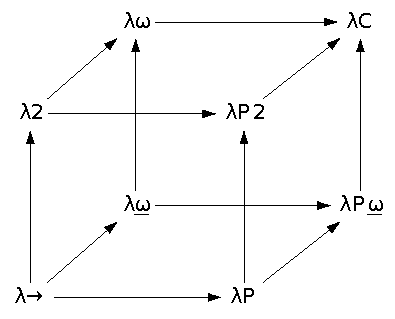
\includegraphics[width=6cm]{assets/Lambda_Cube.pdf}
  \caption{Lambda 方块}\label{fig:lambda-cube}
\end{wrapfigure}

关于不同类型论的表达力，我们可以在 Barendregt 提出的 Lambda Cube 中清晰比较。
从左下角到右上角，这一立方体代表的类型论的表达力逐渐增强，更具体的说，
x 轴的箭头 $\to$ 表示那些类型可以依赖值的类型论，属于依值类型\footnote{即依赖类型，此处为和下文区分做调整。}；
y 轴的箭头 $\uparrow$ 表示项可以依赖类型，即具备多态；
z 轴的箭头 $\nearrow$ 则表示类型可以依赖类型，即具备类型构造子。

在这一立方体中，$\lambda_\to$ 表示简单类型\lambdacalc（simply typed $\lambda$-calculus）、
$\lambda_2$ 表示 System F、$\lambda_\omega$ 表示 System $\mathsf{F}_\omega$\footnote{
  Haskell（GHC）使用这一系统，同时加上 ADT 和 Typal Equality.
}，而位居表达力顶端的类型论则是 Coquand 提出的 Calculus of (inductive) Constructions（$\lambda_\mathsf{C}$），被广泛的运用于
各个定理证明器中，包括 Coq 和 Lean.

而 \Tigris 使用的扩展 HM 系统则处于 $\lambda_\to$ 和 $\mathsf{F}_\omega$ 之间，这是因为我们虽然支持
直谓多态（predicative polymorphism，亦称 rank-1 polymorphism），我们并不支持 arbitrarily ranked 多态，
亦不支持非直谓多态（impredicative polymorphism），不满足 $\mathsf{F}$；此外其虽然支持 HKT，
但并不支持柯里化的类型构造子，因而最相似的类型论应当是 $\mathsf{F}_{\underline\omega}$. 但是即便如此，
我们认为 \Tigris 的类型系统的表达力已经胜过绝大多数具有多态的语言，因为无论是 Arbitrary-Ranked Polymorphism、
Impredicative types 还是 Higher-Kinded Types，都还停留在 PL 学术界阶段，并未得到
大规模的语言的支持。此外，\Tigrisd 的类型系统是 $\lambda_{\Pi\underline\omega}$ 与 $\lambda_{\Pi 2}$的简化混合体，
因为我们并未完全实现主流定理证明器所用的 CIC.

然而，类型论表达力的增强并非没有代价。Hindley-Milner 类型系统之所以经典，不仅仅是因为其开创性，
更因为它小心的设计。事实上，System $\mathsf{F}$ 及以上表达力的系统其
类型推论为不可判定（undecidable）且必须依赖用户的类型标注。对这些系统的推论/检查工作必须在本地通过
双向算法进行（local bidirectional type inference/checking）——即便是类型系统发达的
Haskell，也必须在使用上述高级特性时切换到另一个类型检查器——更不消说依赖类型论。
所以，即便 \Tigris 失去了很大程度的（逻辑上）的表达力，但考虑到本课题的编程子系统并不负责数学证明，
更不希望失去招牌的强大类型推论功能，我们认为这一表达力牺牲是完全值得的。

回到 IR 本身，之所以仍然选用 System $\mathsf{F}$ IR，是基于软件工程的认识：考虑本课题的未来展望，即便之后希望加上
上方的这些功能，我们也不需要耗费精力开展大型重构，可以在现有框架下直接进行补充。

同时，为了方便对编译器做 debug，我们利用与 Wadler 相似的 pretty-printing 算法打印 \texttt{FExpr} AST，
在前文的样例中亦有出现：输出结果与 \Tigris 的一个子集十分相似，同时还会添加必要的类型标注、类型 lambda 抽象与类型应用。
同样的打印算法也用于输出本文之后所描述的所有 IR 和 SBCL 目标代码。

类型系统、类型检查是 \Tigris \emph{极为重要}的组成部分。在下文我们会有更细节的论述。
\section{本章小结}（..略..）